\documentclass[preprint,number]{elsarticle}
\usepackage[utf8]{inputenc}
\usepackage{multirow}
\usepackage{amsthm}
\usepackage{algorithmic}
\usepackage{algorithm}
\usepackage{graphicx}
\usepackage{wrapfig}
\usepackage{appendix}
\usepackage{subcaption}
\usepackage{siunitx}

\usepackage{pdflscape}



\usepackage[draft]{todonotes}
\newcommand{\comment}[1]
{\par {\bfseries \color{blue} #1 \par}} %comment showed

%scientific notation setup
\sisetup{
	round-mode = places,
	round-precision = 2,
	scientific-notation = false}



\usepackage{booktabs}



\usepackage{float}
\floatname{algorithm}{Model}
\newcommand{\algorithmname}{Model}


\newtheorem{mydef}{Definition}

\begin{document}
	\begin{frontmatter}
		
		\author[ul]{Davide Nunes\corref{cor1}}
		\ead{davide.nunes@di.fc.ul.pt}
		\author[ul]{Luis Antunes}
		\ead{xarax@di.fc.ul.pt}
		
		\cortext[cor1]{Corresponding author}
		
		\address[ul]{Group of Studies in Social Simulation (GUESS), Laboratory of Agent Modelling, University of Lisbon, 1749-016 Lisbon, Portugal}
		\title{Modelling Structured Societies: a Multi-relational Approach to Context Permeability}
		
		\begin{abstract}
			The structure of social relations is fundamental for the construction of plausible simulation scenarios. It shapes the way actors interact and create their identity within overlapping social contexts. Each actor interacts in multiple contexts located within relations that constitute their social space. We present a modelling approach to construct structured agent societies with multiple concomitant social networks. We study the notion of context permeability using a consensus game in which agents try to achieve global consensus. We design and analyse two different models of permeability. In the first model agents interact concurrently in multiple social networks. The second model uses a context switching mechanism that adds temporal dynamics to agent interaction. They switch between the different networks spending more or less time in each network. We compare each model and analyse the influence of different social networks in the speed of convergence to consensus. We conduct a series of experiments that show the impact of coexisting social networks when designing simulation models. This approach unveils both the limitations of the current modelling approaches and possible research directions for complex social space simulations.
		\end{abstract} 
		
		\begin{keyword}
			Social Simulation and Modelling \sep Agent Societies \sep Consensus \sep Context \sep Social Networks
		\end{keyword}
		
	\end{frontmatter}
	\newpage
	%******************************************
	%		INTRODUCTION
	%******************************************
	\section{Introduction}
	\label{sec:introduction}
	%******************************************
	%		Research context
	%******************************************
	Studying simulation models of consensus formation can advance our understanding of real-world emergent social phenomena. Typically, we can construct models with different levels of abstraction. Simulation methods can range from data-driven paradigms to more abstract descriptions that allow us to create \textit{what-if-scenarios}. While most models are simplified descriptions of the real-world, many constitute complex systems themselves and thus the necessity of tools like simulation to explore their properties. In \cite{Emmeche1997}, Emmeche makes a distinction between two types of complexity. He characterises the complexity of real systems as \textit{``ontological complexity"} and the one of models as \textit{``descriptive complexity"}. Examples of real-world target phenomena for social simulation models include for instance the joint assessments of policies or, in the context of economics and politics, \textit{the voting problem}. Herbert Simon investigations on this problem were also one of the first stepping stones to the field of social simulation \cite{Simon1954}.
	
	In agent-based \textit{opinion dynamics}, agent interactions are guided by \textit{social space} abstractions. In some models, dimensionality is irrelevant and any agent can interact with any other agents.
	Other approaches use an underlying structure to create agent neighbourhoods. Axelrod for instance, in its model of \textit{dissemination of culture} \cite{Axelrod1997}, represents agents in a bi-dimensional grid. Finally, in an attempt to mimic real social systems, some simulation models make use of \textit{complex network models} (see \cite{Weisbuch2004}) to create the infrastructure that guides agent interaction.
	
	%******************************************
	%		Motivation 
	%******************************************
	%position, most agent-based models don't take into account  social relations and this is important
	In real-world scenarios, actors engage in a multitude of social relations different in kind and quality. Most simulation models don't explore \textit{social space} designs that take into account the differentiation between coexisting social networks. Modelling multiple concomitant relations was an idea pioneered by Peter Albin in \cite{Albin1975} but without any further development. The complex social structures that results from interacting in these different dimensions forms the basis for the formation of social identity \cite{Roccas2002,Ellemers2002}.
	
	%******************************************
	%		Objectives
	%******************************************
	In this paper, we explore the possibility of modelling opinion dynamics with multiple social networks. We look at how the properties influence the convergence to opinion consensus. Starting with this premise of 
	using multiple social networks, we present a series of models that use these networks in different ways which creates distinct emergent dynamics. We want to observe the consequences of using multiple social networks at the same time ---while maintaining the model as simple and abstract as possible much like what happens with the current contributions on opinion dynamics present in the literature. 
	
	In our models agents can: interact at the same time in the multiple networks (choosing partners from any network) or switch between networks (choosing only partners from their current network). While our models seem quite simple, and are quite abstract, they generate quite complex outcomes and thus the need of simulation to understand their dynamics.
	
	%******************************************
	%		Paper Structure
	%******************************************
	\subsection{Paper Structure}
	This paper is organised as follows. In the next section we present work related to, \textit{opinion dynamics}, \textit{social space} modelling and \textit{complex network models}. In the following section, we describe our game of consensus and introduce multiple model variations designed to study the notion of context permeability and the process of consensus formation in multiple social networks. Section \ref{sec:experimental-setup} describes the experimental set-up; the set of tool and methodologies followed to conduct our investigations. In section \ref{sec:results-discussion}, we present and discuss our results and compares the different simulation models. Finally we conclude by making a summary of what we learned from the simulation models and point out possible future research directions.
	
	%******************************************
	%		Related Work
	%******************************************
	\section{Related Work}
	\label{sec:relatedwork}
	%******************************************
	%	Opinion Dynamics
	%******************************************
	\subsection{Opinion Dynamics and Consensus Formation}
	Formal opinion dynamics models provide an understanding if not an analysis of opinion formation processes.  An early formulation of these models was designed to comprehend complex phenomena found empirically in groups \cite{French1956}. In particular, the work on consensus building in the context of decision-making was first studied by DeGroot \cite{Degroot74} and Lehrer \cite{Lehrer1975}. Empirical studies of opinion formation in large populations have methodological limitations, as such, computational sociology arises with a set of tools to cope with those limitations. We use simulation, in particular \textit{multi-agent simulation (MAS)}, as a methodological framework to study such phenomena in a larger scale. Most opinion dynamics simulation models are based either on binary opinions \cite{Galam1997,Antunes2009} or continuous values \cite{Deffuant2000,Deffuant2002}. In these models, agents update their opinions either under social influence or according to their own experience. For a detailed analysis over some opinion dynamics model analytical and simulation results, refer to \cite{Hegselmann2002}.
	
	Opinion dynamics models try to study under which circumstances consensus or polarisation is reached. Agent-based models can have broader applications outside social simulation. In distributed systems in general, consensus is a means by which processes agree on some data value that is needed during computation, typically, this agreement is the result of a negotiation process often with the aid of a mediator. In human societies, social conventions emerge to deal with coordination and subsequently with cooperation problems \cite{Lewis1969}, these conventions are regularities of behaviour that can turn normative with time due to their being persistent solutions to such problems. Moreover, conventions typically originate from the necessity to resolve conflict. MAS can also benefit from being capable of produce emergent conventions in coordination or cooperation problems \cite{Delgado2002}. The decentralised nature of these models of consensus is highly desirable for problems where dynamic control is needed. In these scenarios, creating conventions before hand (off-line) or developing a central control mechanism for generating them can be a difficult and intractable task. MAS can be designed to update their values and strategies based on this local information. Consequently, the guarantee of achieving a global consensus and the efficiency of convergence towards it has been a natural concerns in the design of local interaction behaviours. 
	
	Consensus models are also investigated as means to create conventions in MAS. Shoham and Tennenholtz \cite{Shoham1994} create a bridge between economic literature and machine learning by studying a series of models in which multiple agents are engaged in learning a particular convention. They call this process \textit{co-learning}. The complexity of these systems derives from the its concurrent nature: one agents adapts to the behaviour of another agent it has encountered, as these agents update their behaviour in a similar fashion, this results in a highly non-linear system dynamics. In their work, Shoham and Tennenholtz define the notion of \textit{stochastic social games} and compare different rules with the objective of establishing conventions in a decentralised fashion. In their stochastic games, they present one particular rule which we use in our models: 
	
	\begin{mydef}
		\label{def:external-majority}
		\textit{External Majority (EM)} update rule: adopt action $i$ if so far it was observed in other agents more often than other action and remain with your current action in the case of equality. 
	\end{mydef}
	
	This EM was shown to coincide with \textit{Highest Cumulative Reward (HCR)} which is a simple rule that states that ``an agent should adopt an action that has yielded the highest cumulative reward to date". We chose to use EM in our simulation models for its simplicity and success in the evolution of conventions. We can see that there is an overlap between opinion dynamics from social simulation and agent based learning---or co-learning in this case.
	
	%******************************************
	%	Social Structure in Simulation Models
	%******************************************
	\subsection{Social Structure in Simulation Models}
	One of the most widely used approaches to represent social spaces in abstract simulation models is using a  bi-dimensional gridd. This approach has its origins in the first \textit{“checkerboard”} model introduced in computational social sciences by Thomas Schelling \cite{Schelling1971} and Sakoda \cite{Sakoda1971}. Another famous example that uses bi-dimensional grids as social structure is the social simulation model of dissemination of culture from Axelrod \cite{Axelrod1997}.
	
	Cellular automata (CA) is an example from the are of artificial life that also makes use of bi-dimensional structures to model neighbourhood interactions. While these models are idealised frameworks, the exploration of simple computational models can bring us deeper insights than models with high levels descriptive complexity which would render their analysis, very difficult. The work of Flache and Hegselmann \cite{FlacheHegselmann2001} relaxes the standard CA assumptions about the regular bi-dimensional grids by considering irregular grid structures (Voronoi diagrams). This work presents results on the robustness of some important general properties in relation to variations in the typical grid structure. We can also find contributions that incorporate both the complexity of network models and the behaviour of dynamic processes. One example of this combination is the work in \cite{Sullivan2000} which explores a graph-based cellular automaton to study the relationship between spatial form of urban systems and the robustness of different process dynamics under spatial change. Moreover this allows for the integration of real geographical information to construct the graph-cellular automata. This fact makes so that while the models of dynamic processes are relatively abstract, they are tested in spatial structures based on data from real complex structures and thus making a connection between purely abstract models and data-driven models.
	
	%******************************************
	%	Complex Network Models
	%******************************************
	
	Finally, another type social space models are the \textit{random graph / network models}. Networks with different properties can be built using network models. Each complex network or class of complex networks, presents specific topological features. These properties are typically found in---and the models inspired by---real-world network structures. One of the first complex network models is the random graph from Erdős and Renyi \cite{Erdos1959}. Other examples include the model of preferential attachment \cite{Barabasi1999} and the small-world network models \cite{Watts1998}. One common problem of these models is the fact that once generated, the network structure is static so these models are not really suitable for the description of highly dynamic groups or communities. An example of a model that takes these dynamics into account is the model of team formation~\cite{Gaston2005}. A more in-depth review of network models and their properties is given in~\cite{Nunes2012}.
	
	
	\section{Multi-context Models}
	\label{sec:multi-context-models}
	In this section, we present our modelling approach to explore the concept of permeability between contexts. In our approach, we considers multiple social networks as a way to represent the complex social space of an agent. This setting can be seen in a simulation as a n-dimensional scenario where each dimension surface represents a different social relation (see figure \ref{img:multiple-relations}). Each relation is instantiated using a social network model. The word ``context" is used in many different senses and it is subjected to many analysis \cite{Hayes1997}. Here, we use the term \textit{social context} in a simpler and more strict way. Agents belong to distinct social contexts (neighbourhoods) in these multiple networks. The \textit{social context} of an agent is thus a set of neighbours currently available for interaction. \textit{Context Permeability} is the ability of a particular norm, strategy, opinion or trend to permeate from one social relation to another. Agents belonging to disjoint neighbourhoods in different networks foster the creation of bridges between subsets of the population that wouldn't otherwise be influenced by a consensus formed in a distant coalition or in a distinct context. 
	
	
	
	\begin{figure}[h]
		\centering
		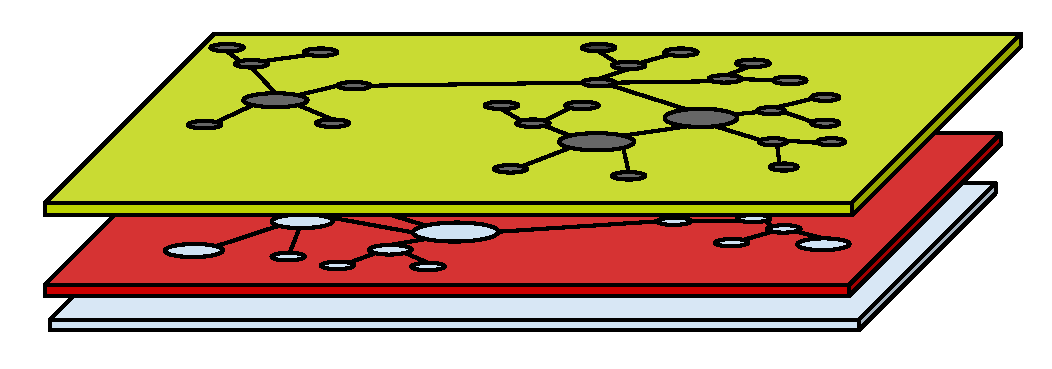
\includegraphics[width=0.7\linewidth]{./images/multi-context_model.pdf}
		\begin{minipage}{0.9\linewidth}
			\caption{Multiple social network structure that shapes the social space in our simulation models.}
			\label{img:multiple-relations}
		\end{minipage}
	\end{figure}
	
	%Consensus
	We study the notion of context permeability in different simulation models in which agents interact using a simple consensus game. The society of agents has to adopt a binary \textquotedblleft option \textquotedblright according to a majority rule. We use the speed of consensus as a measure for self-organisation, exploring the relationship between different network topologies and this measure.
	
	%Presenting 3 models
	We partitioned the design space of our experiments using different simulation models. Each model is designed to analyse different aspects of social context permeability. In a first model \cite{Antunes2007, Antunes2010}, we study the notion of permeability by overlapping social networks. In a second model \cite{Antunes2009}, we analyse the dynamics introduced by switching between \textit{social contexts}(neighbourhoods in different networks), adding a temporal component to neighbourhoods within different social relations. 
	
	\subsection{Simulation and Consensus Game}
	\label{sec:sim_consensus}
	Our agent-based models are designed as \textit{discrete-event} models. On each simulation cycle, every agent executes a simulation step. The agents are selected in a random uniform fashion for execution. This is common practice in agent-based simulation and guarantees that there is no bias caused by the order in which the agents are executed. For each simulation model, we present a description of the individual agent behaviour. Every model we present can be seen as a binary opinion dynamics model or a consensus game. In this game, the society of agents tries to reach an arbitrary global consensus about two possible choices. Each agent keeps track of the number of choices observed from interaction partners throughout a simulation run. In each iteration, each agent selects an available neighbour to interact with and observes its current choice. The agent decides to switch its current choice if the observed option becomes the majority of the two possible choices. The objective of the game is to reach a global consensus, but the particular choice that gets collectively selected is irrelevant. What is important is that overall agreement is achieved. In the consensus game we consider, each agent uses the previously presented external majority (EM) rule to update its opinion value (see definition \ref{def:external-majority} in section \ref{sec:relatedwork}).
	
	
	
	\newpage
	\subsection{Context Permeability}
	This first model of context permeability \cite{Antunes2007,Antunes2010} is designed to study our first setting for permeability. In most interesting applications, an agent is immersed in a complex social world where it engages in a multitude of relations with other agents (and even aggregate agents such as institutions or informal groups). In this model we consider that the \textit{context permeability} is created by agents that can belong simultaneously to several relations. As an example, two agents can be simultaneously family and co-workers, and while some links might not connect two agents directly, others can contain neighbourhoods in which they are related~(either directly or through a common neighbour). Model \ref{model:context_permeability} describes the behaviour of each agent for each simulated step.
	%***************************************************
	%	Context Permeability Model Description
	%***************************************************
	\begin{algorithm}[H]
		\caption{Context Permeability}
		\label{model:context_permeability}
		\algsetup{indent=2em}
		\begin{algorithmic}
			\vspace{0.5em}
			\STATE $M$ \COMMENT{Simulation Model / Environmnet}
			\STATE $A$ \COMMENT{Current Agent in Execution}
			\\ \hrulefill 
			
			\STATE\COMMENT{\textbf{Randomly select a network}}
			\STATE $r$ $\leftarrow$ randomUniform(0,$ M.networks.length() $)
			\STATE network $\leftarrow$ $M.networks[r]$
			
			\STATE
			\STATE \COMMENT{\textbf{Randomly select a neighbour}}
			\STATE neighbours $\leftarrow$ network.neighboursOf($A$) 
			\STATE $r$ $\leftarrow$ randomUniform(0,neighbours.length())
			\STATE partner $\leftarrow$ neighbours[r]
			\STATE
			\STATE \COMMENT{\textbf{Update opinion and memory}}
			\STATE \COMMENT{opinions take the values \{0,1\}--so they can be used as an index}
			\STATE A.memory[partner.opinion]++
			\IF {(A.memory[partner.opinion] $>$ A.memory[A.opinion])}
			\STATE A.opinion $\leftarrow$ partner.opinion
			\ENDIF
		\end{algorithmic}
	\end{algorithm}
	In this model, on each time step, each agent selects a random neighbour from any 
	social network available and updates its opinion based on the opinion of the selected partner using the \textit{external majority} rule. 
	
	
	\subsection{Context Switching}
	\label{sec:models_cs}
	In the context switching model \cite{Antunes2009}, agents are embedded in multiple relations represented as static social networks and they switch \textit{contexts} with some probability $\zeta_{C_i}$ associated with each context $C_i$. The switching probability value is the same in the same network. Each agent switches from its current neighbourhood to a its neighbourhood in another network (in which this agent was inactive). The agents are only active in one context at a time and can only perform encounters with neighbours in the same context. We can think of context switching as a temporary deployment in another place, such as what happens with temporary immigration. The network topology is static; when an agent switches from one network to another, they become inactive in one network and active in their destination. 
	%***************************************************
	%	Context Switching Model Description
	%***************************************************
	\begin{algorithm}[H]
		\caption{Context Switching}
		\label{model:context_switching}
		\algsetup{indent=2em}
		\begin{algorithmic}
			\vspace{0.5em}
			\STATE $M$ \COMMENT{Simulation Model / Environmnet}
			\STATE $A$ \COMMENT{Current Agent in Execution}
			\\ \hrulefill 
			
			\STATE\COMMENT{\textbf{Get the current network (\textit{context} is a network index)}}
			\STATE cNetwork $\leftarrow$ M.networks[A.context]
			\STATE 
			\STATE \COMMENT{\textbf{Get the neighbours for the current network}}
			\STATE neighbours $\leftarrow$ cNetwork.neighboursOf($A$) 
			\STATE \COMMENT {filter by agents active in the same network}
			\STATE neighbours $\leftarrow$ \{n $|$ n $\in$ neighbours $\wedge$ (n.context = A.context)\}
			\STATE
			\STATE\COMMENT{\textbf{Randomly select a neighbour}} 
			\STATE $r$ $\leftarrow$ randomUniform(0,neighbours.length())
			\STATE partner $\leftarrow$ neighbours[r]
			\STATE
			\STATE \COMMENT{\textbf{Update opinion and memory}}
			\STATE \COMMENT{opinions take the values \{0,1\}--so they can be used as an index}
			\STATE A.memory[partner.opinion]++
			\IF {(A.memory[partner.opinion] $>$ A.memory[A.opinion])}
			\STATE A.opinion $\leftarrow$ partner.opinion
			\ENDIF
			\STATE
			\STATE \COMMENT{\textbf{Switch to another network}}
			\STATE switchingProb $\leftarrow$ M.params.switchingProb(A.context)
			\STATE $r \leftarrow $ randomUniform(0,1)
			\IF{($r < $ switchingProb)}
			\STATE numNets $\leftarrow$ M.networks.length()
			\STATE nextNetworks $\leftarrow$ \{i $|$ (i $\in$ [0,numNets[) $\wedge$ (M.networks[i] != A.context)\}
			\STATE $r$ $\leftarrow$ randomUniform(0,nextNetworks.length())
			\STATE A.context $\leftarrow$ nextNetworks[r]
			\ENDIF
		\end{algorithmic}
	\end{algorithm}
	\noindent In this model agents select an (active) partner from their current neighbourhood. If a partner is available the agents update their opinion value based on EM. At the end of the interaction, the agent switches \textit{from} the current context to a different one with a probability associated with its current network. 
	
	This model describes an abstract way to represent the time spent on each network using the switching probability $\zeta_{C_i}$. Here, the permeability between contexts is achieved using this temporal component. Context switching introduces one notion that has not been explored in the literature so far: the fact that, although some social contexts can be relatively stable if we consider short to moderate periods of time, our social peers are not always available at all times and spend different amounts of time in distinct social contexts.
	
	\section{Experimental Setup}
	\label{sec:experimental-setup}
	In this section we describe all the tools and processes necessary to produce the current research output. The experiments for our previously described simulation models were developed using the MASON~\cite{Luke2005} simulation framework written in Java. All the code for the simulation models can be found here \cite{Nunes:Software:11067}. Moreover, all the results presented in this paper were made reproducible by using the \textit{statistical computing language R} \cite{R2008} and the R package \textit{knitr} \cite{knitr2014}. Knitr is used for generating reports that contain the code, the results of its execution (plots and tables), and the textual description for such results. All the R code and the configuration files used to produce the analysed data can be found \textbf{in}...\todo{Archive the data, analysis and code used for the analysis, get a doi for it and cite it here}.

%recap
For each configuration in our experiments we performed 100 independent simulation runs. The results are thus analysed in terms of value distribution, average and standard deviation, or variance over the 100 runs. Like we described in section \ref{sec:sim_consensus}, our models are discrete-event models and each cycle agents execute 
a step in a random order : this is so that this dynamic system --our simulation model-- is not influenced by the order in which agents are executed. Simulations ends when total consensus is achieved or 2000 steps have passed.  

\subsection{Social Network Models}
\label{sec:exp-setup_network_models}
The social networks used in our models are \textit{k-regular} and \textit{scale-free}. A k-regular network is a network where each node has the same number of connections. These networks are constructed by arranging the nodes in a ring and connecting each node to their next $k$ neighbours. Each network has $2k$ edges per vertex. 

Scale-free networks \cite{Barabasi1999} are created with a model of preferential attachment proposed by Barab\'{a}si and colleagues \cite{Barabasi1999}. This model builds upon the perception of a common property of many large networks, a scale-free-power-law distribution of node connectivity. This feature was found to be a consequence of two generic mechanisms: networks expand continuously by the addition of new vertices, and new vertices attach preferentially to sites that are already well connected, being this mechanism more commonly known as ``preferential attachment''. In these networks, the probability $P(k)$ of two nodes being connected to each other decays as a power law, following $P(k) \sim k^{- \gamma}$.

The network instances were generated using the \textit{b-have network library} \cite{Nunes:Software:11069}. This is a Java library which allows for the manipulation of Network/Graph data structures. It also includes the more commonly used random network models from the literature. 

\subsection{Measuring Network Properties}
We measure two structural properties of our networks: the \textit{average path length} and the \textit{clustering coefficient}. The \textit{average path length} measures the typical separation between two vertices in the graph. The \textit{clustering coefficient} measures the average cliquishness of the graph neighbourhood. This measure quantifies how close the neighbours of a node are to forming a clique. Duncan J. Watts and Steven Strogatz \cite{Watts1998} introduced the measure to characterise a class of complex networks called small-world networks. The networks produced by the \textit{b-have network library} \cite{Nunes:Software:11069} were exported to files and analysed using the \textit{igraph R package} \cite{igraph2006}. 

\section{Results and Discussion}
\label{sec:results-discussion}

% Overview

\subsection{Overlapping Network Properties}
\label{sec:network_properties}
In this first analysis, we investigate the properties of different network topologies that we use in our models. 
One of the parameters in some experiments is the number of networks in which the agents interact. Adding more networks means adding more connections. 
We show that what is important is not just the the number of connections, but the properties the resulting structure displays when these networks are merged. The way we look at the network properties is as follows.

Each network is generated in such a way that the node positions are randomised. What this means is that we can have multiple networks with the same topology and yet, each node has a different neighbourhood on each network. Also, neighbourhoods do not necessarily overlap due to the node shuffling. Adding more networks to the social space is not the same as creating a single network with twice the number of connections. 

\noindent Consider figure \ref{fig:network_properties_merge_2_10regular}. We created two random k-regular networks with k=10 and merged them ignoring edges from common neighbours --in the simulation models this edge agglutination is not performed, we use it here for the purposes of network analysis. The common edges are highlighted in a different colour.

\begin{figure}
	\centering
	\includegraphics[width=1\linewidth]{"../analysis/pdf/ network_properties_merge_2_10regular"}
	\begin{minipage}{0.9\textwidth}
		\caption{Overlapping of two k-regular networks, each with k=10.}
		\label{fig:network_properties_merge_2_10regular}
	\end{minipage}
\end{figure}

\begin{table}
	\centering
	\begin{minipage}{0.9\textwidth}
		\caption{Properties for overlapping of two k-regular networks, each with k=10.}
		\label{tab:network_properties_merge_2_10regular}
	\end{minipage}
	\begin{tabular}{lcccc}
		& Nodes &  Edges & Clustering Coef.	  &  Avg. Path Length \\ 
		\hline  10-Regular 1 & 100 &  1,000  &  0.711 &  2.980 \\ 
		\hline  10-Regular 2 & 100 & 1,000 & 0.711 &  2.980 \\ 
		\hline  Combined & 100 & 1,790  & 0.512 &  1.638 \\ 
		\hline 20-Regular & 100 & 2,000	& 0.731	& 1.788 \\
		\hline 
	\end{tabular} 
\end{table}

The networks are drawn using the \textit{Kamada-Kawai} Layout \cite{Kamada19897} which regards the desirable ``geometric" (Euclidean) distance between two vertices in the drawing as the ``graph theoretic" distance between them in the corresponding graph. We can see by the results of the layout in figure \ref{fig:network_properties_merge_2_10regular}, that the distance between nodes in the network has decreased, this is also confirmed by the reduced average path length of the combined networks (see table \ref{tab:network_properties_merge_2_10regular}). 

\begin{wrapfigure}{r}{0.45\linewidth}
	\includegraphics[width=1\linewidth]{"../analysis/pdf/ network_properties_1_20regular"}
	\begin{minipage}{0.8\linewidth}
		\caption{Single k-regular network with k=20. (Drawn using the Kamada-Kawai layout)}
		\label{fig:network_properties_1_20regular}
	\end{minipage}
\end{wrapfigure}

To illustrate our point we analysed one k-regular network with k = 20 (see figure \ref{fig:network_properties_1_20regular} --and the corresponding entry on table \ref{tab:network_properties_merge_2_10regular}). The clustering coefficient of a 20-Regular network is approximately the same as the one of a 10-regular network (higher than the combination of 10-regular networks). The average path length also decreases as there are more connections between the nodes. As we will show, these properties may vary. Since the nodes are subjected to random permutations, we can generate different overlaps which lead to distinct structural values.

Since we model the agent social space as a multitude of networks, we need to investigate the properties resulting from the merging of these networks. We do this empirically by taking the network instances used in the simulation and analysing the distribution of clustering coefficient and average path length for the different configurations.

\subsubsection{Properties of Overlapping K-Regular Networks}
\label{sec:overlapping_kreg}
We will now investigate, what kind of properties we can get from merging K-Regular networks. First, we analysed the distribution for the average path length and the clustering coefficient values over 100 network instances with 100 nodes each. Since this variation is negligible we use the average as a descriptor for different configurations of k values and number of overlapping networks. (The reader should refer to figures \ref{append_fig:network_properties_apl_kreg} and \ref{append_fig:network_properties_cc_kreg} in the appendix for the box plot preliminary analysis.)  

Figure~\ref{fig:network_properties_apl_line_kreg} shows the average value for the \textit{average path length} of 100 k-regular network instances, each with 100 nodes. We can see that the \textit{average path length} changes more drastically when we go from 1 to 2 networks this is precisely the effect we can see in figure \ref{fig:network_properties_merge_2_10regular}. What we are seeing is that merging these networks at random effectively creates multiple shortcuts between points that were not connected in the original k-regular topology. Beyond this point, adding more networks does not modify this structural property in a significant way. Note that, since each network has 100 nodes, with $k=50$ the network is fully connected (hence the average path length being 1). 

\begin{figure}[H]
	\centering
	\begin{subfigure}{.5\linewidth}
		\centering
		\includegraphics[width=1\linewidth]{"../analysis/pdf/ network_properties_apl_line_kreg_12345"}
		\caption{}
		\label{fig:network_properties_apl_line_kreg_12345}
	\end{subfigure}%
	\begin{subfigure}{.5\linewidth}
		\centering
		\includegraphics[width=1\linewidth]{"../analysis/pdf/ network_properties_apl_line_kreg_1020304050"}
		\caption{}
		\label{fig:network_properties_apl_line_kreg_1020304050}
	\end{subfigure}
	\begin{minipage}{0.9\textwidth}
		\vspace{0.2cm}
		\caption{Average value for the \textit{average path length} of 100 instances of overlapping k-regular networks(containing 100 nodes each) with ~k=\{1,2,3,4,5\}~(\ref{fig:network_properties_apl_line_kreg_12345}), and k= ~\{10,20,30,40,50\} (\ref{fig:network_properties_apl_line_kreg_1020304050}).}
		\label{fig:network_properties_apl_line_kreg}
	\end{minipage}
\end{figure}

\noindent Figure~\ref{fig:network_properties_cc_line_kreg} shows the results for the average \textit{clustering coefficient} of 100 instances of overlapping k-regular networks. We can see that adding multiple networks changes the clustering coefficient of the resulting structure. We can see that for $k \le 20$ the clustering coefficient drops when we add a second network. This happens because when we merge these networks, their connectivity is not enough to generate shortcuts with tightly clustered neighbourhoods. The clustering coefficient is computed by taking the average local clustering coefficient of each node in the network. An initial highly clustered k-regular network (with all the nodes having the same structure) is affected when you modify the node neighbourhoods in such a way that some are more clustered than others.

\begin{figure}[H]
	\centering
	\begin{subfigure}{.5\linewidth}
		\centering
		\includegraphics[width=1\linewidth]{"../analysis/pdf/ network_properties_cc_line_kreg_12345"}
		\caption{}
		\label{fig:network_properties_cc_line_kreg_12345}
	\end{subfigure}%
	\begin{subfigure}{.5\linewidth}
		\centering
		\includegraphics[width=1\linewidth]{"../analysis/pdf/ network_properties_cc_line_kreg_1020304050"}
		\caption{}
		\label{fig:network_properties_cc_line_kreg_1020304050}
	\end{subfigure}
	\begin{minipage}{0.9\textwidth}
		\vspace{0.2cm}
		\caption{Average value for the \textit{clustering coefficient} of 100 instances of overlapping k-regular networks(containing 100 nodes each) with ~k=\{1,2,3,4,5\}~(\ref{fig:network_properties_cc_line_kreg_12345}), and  k = \{10,20,30,40,50\} (\ref{fig:network_properties_cc_line_kreg_1020304050}).}
		\label{fig:network_properties_cc_line_kreg}
	\end{minipage}
\end{figure}

The exception is when you merge networks with $k=1$. These have a ring-like structure so there are no nodes forming a clique\footnote{A clique is a group of nodes such that every two nodes are connected by an edge.} with their neighbours. 

\subsubsection{Properties of Overlapping Scale-free Networks}
In a preliminary analysis we looked at the distribution of property values that results from merging scale-free networks (see figure \ref{append_fig:network_properties_sf}). Like in the previous results, the properties don't vary much between the 100 different instances of each overlapping network configuration. We can then say that specific configurations display a specific \textit{average path length} and \textit{clustering coefficient} both for \textit{k-regular} networks and \textit{scale-free} networks. Since the average of these measures is still a good descriptor, we ploted the average of the \textit{average path length} (figure \ref{fig:network_properties_apl_line_sf_12345}) and \textit{clustering coefficient} (figure \ref{append_fig:network_properties_cc_sf_12345}) for each overlapping network configuration.

\begin{figure}[H]
	\centering
	\begin{subfigure}{.5\linewidth}
		\centering
		\includegraphics[width=1\linewidth]{"../analysis/pdf/ network_properties_apl_line_sf_12345"}
		\caption{}
		\label{fig:network_properties_apl_line_sf_12345}
	\end{subfigure}%
	\begin{subfigure}{.5\linewidth}
		\centering
		\includegraphics[width=1\linewidth]{"../analysis/pdf/ network_properties_cc_line_sf_12345"}
		\caption{}
		\label{fig:network_properties_cc_line_sf_12345}
	\end{subfigure}
	\begin{minipage}{0.9\textwidth}
		\vspace{0.2cm}
		\caption{Average value for the \textit{average path length} (\ref{append_fig:network_properties_apl_sf_12345}) and \textit{clustering coefficient} (\ref{append_fig:network_properties_cc_sf_12345}) for 100 instances of overlapping \textit{scale-free} networks(containing 100 nodes each).}
		\label{fig:network_properties_line_sf}
	\end{minipage}
\end{figure}

The parameter $d$ in figure \ref{fig:network_properties_line_sf} dictates how many edges are added by preferential attachment (see sectino \ref{sec:exp-setup_network_models}) each time a new node is added to a network (during its construction). This means that for $d=1$, the resulting network is a \textit{forest}: a network composed of disjoint tree graphs. Figure~\ref{fig:network_properties_apl_line_sf_12345} shows us that the \textit{average path length} still decreases consistently when we more networks. One of the characteristics of \textit{scale-free} networks is its short average  path length, thus, for $d \ge 2$ we can see that adding more edges does not make so much difference. Scale-free networks also have a reduced \textit{clustering coefficient} which is evident in figure \ref{fig:network_properties_cc_line_sf_12345}. This is increased when we merge more networks.


\subsubsection{Merging K-Regular with Scale-Free Networks}
Finally, we look at what happens when we merge k-regular networks with \textit{scale-free} networks. We didn't make an exhaustive analysis for this configuration but we show what is the resulting structure of such merging. You can see in figure \ref{fig:network_properties_merge_regular_scale-free} that this results in a network with a lower \textit{average path length} due to the shortcuts created by the \textit{scale-free} network. It is also less dense than the structure with two 10-regular networks (figure \ref{fig:network_properties_merge_2_10regular}). In this analysis we consider only the merging of two networks.

\begin{figure}[H]
	\centering
	\includegraphics[width=1\linewidth]{"../analysis/pdf/ network_properties_10regular_2scale-free"}
	\begin{minipage}{0.9\textwidth}
		\caption{Overlapping of a 10-regular with a \textit{scale-free} network with D=2.}
		\label{fig:network_properties_merge_regular_scale-free}
	\end{minipage}
\end{figure}

\begin{figure}[H]
	\centering
	\begin{subfigure}{.5\linewidth}
		\centering
		\includegraphics[width=1\linewidth]{"../analysis/pdf/ network_properties_apl_line_sf_kreg_12345"}
		\caption{}
		\label{fig:network_properties_apl_line_sf__kreg_12345}
	\end{subfigure}%
	\begin{subfigure}{.5\linewidth}
		\centering
		\includegraphics[width=1\linewidth]{"../analysis/pdf/ network_properties_apl_line_sf_kreg_1020304050"}
		\caption{}
		\label{fig:network_properties_apl_line_sf_kreg_1020304050}
	\end{subfigure}
	\begin{minipage}{0.9\textwidth}
		\vspace{0.2cm}
		\caption{Average \textit{average path  length} for 100 instances of heterogeneous network configurations:  1 \textit{scale-free} with $d=\{1,2,3,4,5\}$ and 1 \textit{k-regular} network with $k=\{1,2,3,4,5\}$ (\ref{fig:network_properties_apl_line_sf__kreg_12345}) and $k=\{10,20,30,40,50\}$ (\ref{fig:network_properties_apl_line_sf_kreg_1020304050}). (See the respective box plots in the appendix: figure \ref{append_fig:network_properties_apl_sf_kreg}).}
		\label{fig:network_properties_line_apl_sf_kreg}
	\end{minipage}
\end{figure}

Figure \ref{fig:network_properties_line_apl_sf_kreg} shows the \textit{average path length} of 100 independently generated instances of combinations of 1 \textit{k-regular} network and 1 \textit{scale-free} network with different values $k$ and $d$ respectively. We can see that for configurations where the \textit{k-regular} networks have low values of $k$ (figure \ref{fig:network_properties_apl_line_sf__kreg_12345}), adding a \textit{scale-free} network always decreases the \textit{average path length}. Moreover the higher the $d$ the lower the path length as more connections are formed between different nodes. Which higher values of $k$ (figure \ref{fig:network_properties_apl_line_sf_kreg_1020304050}) however, increasing the value of $d$ does not decrease the \textit{average path length}. This is not surprising given that with that level of connectivity having a more connected \textit{scale-free} doesn't make such an impact. The first network is already highly dense and connected so adding a few extra connections doesn't matte --what matters in this case is that there is a scale-free network creating the extra shortcuts between nodes that weren't connected before.

\begin{figure}[H]
	\centering
	\begin{subfigure}{.5\linewidth}
		\centering
		\includegraphics[width=1\linewidth]{"../analysis/pdf/ network_properties_cc_line_sf_kreg_12345"}
		\caption{}
		\label{fig:network_properties_cc_line_sf__kreg_12345}
	\end{subfigure}%
	\begin{subfigure}{.5\linewidth}
		\centering
		\includegraphics[width=1\linewidth]{"../analysis/pdf/ network_properties_cc_line_sf_kreg_1020304050"}
		\caption{}
		\label{fig:network_properties_cc_line_sf_kreg_1020304050}
	\end{subfigure}
	\begin{minipage}{0.9\textwidth}
		\vspace{0.2cm}
		\caption{Average \textit{clustering coefficient} for 100 instances of heterogeneous network configurations:  1 \textit{scale-free} with $d=\{1,2,3,4,5\}$ and 1 \textit{k-regular} network with $k=\{1,2,3,4,5\}$  (\ref{append_fig:network_properties_cc_sf_12345}) and $k=\{10,20,30,40,50\} $ (See the respective box plots in the appending: figure\ref{append_fig:network_properties_cc_sf_kreg}).}
		\label{fig:network_properties_line_cc_sf_kreg}
	\end{minipage}
\end{figure}

\noindent Figure \ref{fig:network_properties_line_cc_sf_kreg} show the results for the \textit{clustering coefficient}. These are similar to the results we get for \textit{k-regular} networks (see figure \ref{network_properties_cc_line_kreg}). the difference is that we are not adding more networks but rather increasing the parameter $d$ of the scale-free. Curiously in this case, the effects are qualitatively similar with the ones of merged \textit{k-regular} network with low value of $k$. With high values of $k$ (figure \ref{fig:network_properties_cc_line_sf_kreg_1020304050}) we can see that higher values of $d$ are not enough to make the network more clustered. This is because, scale-free networks are more sparse and have a very low number of triangles between nodes.

%***************************************************
%	Context Permeability 
%***************************************************
\subsection{Context Permeability}
\label{sec:results:context_permeability}

In this section, we discuss the results for various set of experiments on the first model we presented --the \textit{context permeability model} \cite{Antunes2007,Antunes2010}. In a first set of experiments, the agent space was structured using \textit{k-regular} and \textit{scale-free }social networks. Each network layer was configured with the same topology. We analyse the context permeability model in terms of convergence to consensus: the ratio of simulations that converged to total consensus over 3000 runs; and how many agent encounters were needed for this to happen. 

\subsubsection{Convergence Ratio}
\label{sec:ctx_perm_convergence}
In this section we analyse the ratio of convergence to consensus for different network configurations. We correlate this ratio with the properties that the combined network structure exhibits. As we have seen in section \ref{sec:network_properties}, the properties don't vary much for different random network instances so we use the average as the descriptor for these properties in this correlation.

The following tables show the results of our simulations. Table ~\ref{tab:regular_convergence} show the percentage of total consensus achieved within 2000 cycles for 3000 runs. We can see that for k-regular networks with a small $k$, consensus is rarely achieved with a single network. However, as soon as we add more networks, consensus is achieved in a significantly greater number of occasions. These results are especially interesting for the \textit{scale-free }networks (table \ref{tab:scale-free_convergence}): as soon as we add more planes, for a \textit{scale-free} with $d\ge2$, we can achieve consensus in a lot of occasions. This is to show that achieving consensus is not just a matter of connectivity. With \textit{scale-free} networks, we can achieve consensus more often with less clustered networks. This convergence is achieved not because of the clustering coefficient but rather due to lower \textit{average path length}. This is difficult to visualise using only the tables and the previous plots so, to confirm this hypothesis, we measured the \textit{Spearman's correlation} between the ratio of convergences to consensus, the average of \textit{average path length} , and the average of \textit{clustering coefficient} for the corresponding network configurations (see table \ref{tab:convergence_correlation}).

\begin{table}[H]
	\centering		
	\begin{minipage}{0.9\textwidth}
		\caption{Ratio of convergence to total consensus in 3000 independent runs with with a number of concomitant networks ($\#$ nets.) equal in kind: k-regular networks with $k=\{1,2,3,4,5,10,20,30,40,50\}$.}
		\label{tab:regular_convergence}
	\end{minipage}
	
	
	\setlength{\tabcolsep}{.30000em}
	\begin{tabular}{c|SSSSSSSSSS}
		
		\toprule
		& \multicolumn{10}{c}{value for k} \\ 
		\# nets.  & 1 & 2 & 3 & 4 & 5 & 10 & 20 & 30 & 40 & 50\\
		\midrule
		1  & 0.0000 & 0.0000 & 0.0006667 & 0.0050  & 0.01633 & 0.1830 & 0.6713 & 0.9673 & 1.0000 & 1.0000 \\
		2  & 0.0770 & 0.5887 & 0.8136667 & 0.8967 & 0.93467 & 0.9817 & 0.9977 & 1.0000 & 1.0000 & 1.0000 \\
		3  & 0.6560 & 0.9417 & 0.9780000 & 0.9920 & 0.99433 & 0.9997 & 1.0000 & 1.0000 & 1.0000 & 1.0000 \\
		4  & 0.8780 & 0.9867 & 0.9966667 & 0.9993 & 1.00000 & 1.0000 & 1.0000 & 1.0000 & 1.0000 & 1.0000 \\
		5  & 0.9497 & 0.9937 & 0.9993333 & 1.0000 & 1.00000 & 1.0000 & 1.0000 & 1.0000 & 1.0000 & 1.0000 \\
		\bottomrule
	\end{tabular}
\end{table}


\begin{table}[H]
	\centering
	\begin{minipage}{0.9\textwidth}
		\caption{Ratio of convergence to total consensus in 3000 independent runs with a number of concomitant networks ($\#$ nets.) equal in kind: \textit{scale-free} networks with $d=\{1,2,3,4,5\}$.}	
		\label{tab:scale-free_convergence}
	\end{minipage}
	
	\setlength{\tabcolsep}{.30000em}
	\begin{tabular}{c|SSSSS}
		\toprule
		& \multicolumn{5}{c}{value for d} \\ 
		$\#$ nets.  & 1 & 2 & 3 & 4 & \multicolumn{1}{c}{5} \\ 
		\midrule
		1  &  0.0000  &  0.2903  &  0.8590  &  0.9573  &  0.9873  \\
		2  &  0.2840  &  0.9287  &  0.9877  &  0.9973  &  0.9980  \\
		3  &  0.7793  &  0.9850  &  0.9970  &  1.0000  &  1.0000  \\
		4  &  0.9287  &  0.9977  &  0.9997  &  1.0000  &  1.0000  \\
		5  &  0.9737  &  0.9997  &  1.0000  &  1.0000  &  1.0000  \\
		\hline 
	\end{tabular}
\end{table}

\begin{table}[H]
	\caption{Spearman's correlation between convergence ratio (CR), average \textit{average path length} (APL) and \textit{clustering coefficient} (CC) along with the respective p-value and confidence interval, for a confidence level of 95\%.}
	\label{tab:convergence_correlation}
	
	
	\centering	
	\begin{tabular}{r|cc|cll}
		
		\toprule
		network model & X & Y & Correlation & CI(95\%) & p-value \\
		\midrule
		k-regular & CR & APL & -0.726 & [-0.836, -0.561] & \num[scientific-notation = true]{2.437e-09} \\
		k-regular & CR & CC & 0.264   &   [-0.015,  0.505]       &    \num[scientific-notation = true]{0.064}     \\
		\midrule
		scale-free & CR & APL &    -0.912     &  [-0.961, -0.808]       &   \num[scientific-notation = true]{2.28e-10} \\
		scale-free & CR & CC & 0.633   &   [0.318, 0.823]  &   \num[scientific-notation = true]{0.0006776} \\
		\hline
		
		\hline
	\end{tabular}
\end{table}

\subsubsection{Number of Encounters to Achieve Consensus}
\label{sec:ctx_perm_encounters}
We now analyse the convergence in terms of average number of meetings during a simulation run. Since the maximum number of simulation cycles is 2000, the maximum number of encounters is 2000000 (we have 100 agents and each one performs 1 encounter per cycle). We show that for some configurations, the average of encounters is not a good descriptor since it varies greatly from run to run. It is better to look at the distributions of these measures rather than considering the average. Nevertheless, we included the data with all the average number of encounters as well as the respective standard deviations for different network configurations. You can find this data in appendix \ref{append_ctx_permeability}.

%boxplots for k-regular networks
First, we present the results for k-regular networks. In the box plots To observe the distribution of the number of encounters consider the box plots for $k = \{1,2,3,4,5\}$ (figure \ref{fig:ctx_perm_kreg_12345}) and $k =\{10,20,30,40,50\}$ (figure \ref{fig:ctx_perm_kreg_1020304050}). In figure \ref{fig:ctx_perm_kreg}, we focus on configurations with a number of networks $\ge 3$ since less networks lead to much worse results in terms of convergence speed. These plots still present two types of situations: the typical runs in which the number of encounters doesn't vary that much and some ``outlier runs" which present some interesting dynamics as we will see later.

\begin{figure}[H]
	\centering
	\begin{subfigure}{.49\linewidth}
		\centering
		\includegraphics[width=1\linewidth]{"../analysis/pdf/ context_permeability_encounters_kregular_12345"}
		\caption{}
		\label{fig:ctx_perm_kreg_12345}
	\end{subfigure}%
	\begin{subfigure}{.49\linewidth}
		\centering
		\includegraphics[width=1\linewidth]{"../analysis/pdf/ context_permeability_encounters_kregular_1020304050"}
		\caption{}
		\label{fig:ctx_perm_kreg_1020304050}
	\end{subfigure}
	\begin{minipage}{0.9\linewidth}
		\vspace{0.2cm}
		\caption{Number of meetings over 100 independent simulation runs for multiple k-regular networks: $k=\{1,2,3,4,5\}$~(\ref{fig:ctx_perm_kreg_12345}) and $k=\{10,20,30,40,50\}$~(\ref{fig:ctx_perm_kreg_1020304050})).}
		\label{fig:ctx_perm_kreg}
	\end{minipage}
\end{figure}

\noindent Figure~\ref{fig:ctx_perm_kreg} shows us results that are qualitatively similar to what we previously observed for convergence ratios (see section \ref{sec:ctx_perm_convergence}). Networks with less connectivity and a greater average path length lead to total convergence less often. Moreover, the simulation outcomes vary much more in comparison with the other configurations ($k>1$ and $networks \ge 3$).

Notice that for $k=3$ and $networks=3$ (\ref{fig:ctx_perm_kreg_1020304050}), we still have runs that deviate from what we consider the typical behaviour. Instead of disregarding this as a simple outlier, we show that this run allows us to gain an insight on the dynamics of our \textit{External Majority} consensus game.

Before anything else we analysed the network structure from this run and observed that there were no distinct differences between the network instances from the ``outlier run" and the ones of the ``typical" run. This suggested that this can be a property of the game itself --and of the network structure that leads to this situation -- and what happens is that the agents reach a state from which converging towards consensus is significantly harder. Villatoro \cite{Villatoro2013}  found that some complex network models lead consensus games to form metastable sub-conventions. These are very difficult to break and reaching 100\% agreement is not as straightforward as assumed by previous researchers. We are not concerned with this difficulty but rather with what happens in similar cases. Figure~\ref{fig:ctx_perm_kreg_runs} shows the consensus progression for two simulation runs a typical case and the outlier.

\begin{figure}[H]
	\centering
	\begin{subfigure}{.49\linewidth}
		\centering
		\includegraphics[width=1\linewidth]{"../analysis/pdf/ context_permeability_simrun_kregular_k10_normal"}
		\caption{Typical Run}
		\label{fig:ctx_perm_kreg_run_normal}
	\end{subfigure}%
	\begin{subfigure}{.49\linewidth}
		\centering
		\includegraphics[width=1\linewidth]{"../analysis/pdf/ context_permeability_simrun_kregular_k10_outlier"}
		\caption{Outlier Run}
		\label{fig:ctx_perm_kreg_run_outlier}
	\end{subfigure}
	
	\begin{minipage}{0.9\linewidth}
		\vspace{0.2cm}
		\caption{Number of agents with each opinion during a simulation run: typical run in \ref{fig:ctx_perm_kreg_run_normal} and ``outlier run" in \ref{fig:ctx_perm_kreg_run_outlier}.}
		\label{fig:ctx_perm_kreg_runs}
	\end{minipage}
\end{figure}


\noindent In our case, we take the outlier in the configuration with $k=3$ and $networks=3$ and look at the memory that agents use in the consensus game. As we described previously, agents record the number of individuals encountered with each opinion value (two opinions in this case). We look at the average difference between the number of opinions observed for all the agents. We also look at the variance to see if the opinion observations evolve in an uniform fashion throughout the simulation. Figure~\ref{fig:ctx_perm_kreg_runs_diff} shows the average difference between opinion memory for the first 10 steps (which was when the simulation converged for the normal run).

\begin{figure}[H]
	\centering
	\begin{subfigure}{1\linewidth}
		\centering
		\includegraphics[width=1\linewidth]{"../analysis/pdf/ cp-regular-normal-run-memory-diff"}
		\caption{Typical Run}
		\label{fig:ctx_perm_kreg_run_normal_diff}
	\end{subfigure}%
	\\
	\begin{subfigure}{1\linewidth}
		\centering
		\includegraphics[width=1\linewidth]{"../analysis/pdf/ cp-regular-outlier-run-memory-diff"}
		\caption{Outlier Run}
		\label{fig:ctx_perm_kreg_run_outlier_diff}
	\end{subfigure}
	
	\begin{minipage}{0.9\linewidth}
		\vspace{0.2cm}
		\caption{Average and variance of the difference between opinions observed for the 100 agents: typical run in figure \ref{fig:ctx_perm_kreg_run_normal_diff} and first steps of the``outlier run" in figure \ref{fig:ctx_perm_kreg_run_outlier_diff}.}
		\label{fig:ctx_perm_kreg_runs_diff}
	\end{minipage}
\end{figure}

We can see that both the average difference in the opinion memory and the variance, rise faster in the normal run than it does in the outlier run. This is not enough to establish that there is a significant difference between the two. Moreover, the memory differences are quite similar but the number of agents for each opinion was quite even. This happens due to the position of agents in the network and their initial opinion values. These circumstances led the agents to a initial stability. Note that the opinion difference continues to rise throughout the simulation along with the variance. The variance starts to increase more rapidly after 200 steps. The exponential growth reveals that the convergence to consensus is not done evenly throughout the network, this is one of the reasons why consensus takes more time to achieve. Also, the low variance in the first $200$ steps shows us that the opinion strength was evenly distributed --we have almost the same number of agents for each opinion but the memory differences are qualitatively the same for both opinions. As soon as this variance increases, one of the opinions breaks the stable state and the convergence towards global consensus begins. 

\begin{figure}[H]
	\centering
	\includegraphics[width=1\linewidth]{"../analysis/pdf/ cp-regular-outlier-fullrun-memory-diff"}
	\begin{minipage}{0.9\textwidth}
		\caption{Average and variance of the difference between opinions observed for the 100 agents throughout the outlier run.}
		\label{fig:ctx_perm_kreg_run_outlier_diff_full}
	\end{minipage}
\end{figure}

\noindent In other words, in some sections of the network, the agents converged towards one opinion and continue to reinforce each other (leading the opinion difference to grow) and the more regions converge, the faster the global convergence is.  
%boxplots for scale-free networks

\begin{figure}[H]
	\centering
	\begin{subfigure}{.49\linewidth}
		\centering
		\includegraphics[width=1\linewidth]{"../analysis/pdf/ context_permeability_encounters_sf"}
		\caption{}
		\label{fig:ctx_perm_sf_full}
	\end{subfigure}%
	\begin{subfigure}{.49\linewidth}
		\centering
		\includegraphics[width=1\linewidth]{"../analysis/pdf/   context_permeability_encounters_sf_best"}
		\caption{}
		\label{fig:ctx_perm_sf_best}
	\end{subfigure}
	\begin{minipage}{0.9\linewidth}
		\vspace{0.2cm}
		\caption{Number of meetings over 100 independent simulation runs for multiple \textit{scale-free} networks: with d=\{1,2,3,4,5\} (\ref{fig:ctx_perm_sf_full}) with a zoom on the best configurations in \ref{fig:ctx_perm_sf_best}.}
		\label{fig:ctx_perm_sf}
	\end{minipage}
\end{figure}


\noindent Figure~\ref{fig:ctx_perm_sf} shows the average number of encounters during 100 independent simulation runs for \textit{scale-free} networks. (We don't include the configuration for 1 network and $d = 1$ because as we have seen in the convergence results, these never converge. The convergence ratio is very low for the configurations with 1 network $d = 2$ and 2 networks with $d = 1$; hence the high number of encounters~(see also table \ref{tab:scale-free_convergence}).

These results are similar to those of \textit{k-regular} in that adding more networks speeds up the convergence to consensus. The difference is that more ``atypical" runs occur with multiple \textit{scale-free} networks. Again, this is the effect ot these types of topologies. As we discussed previously, in these less connected topologies, agents are more prone to be arranged in such a way that progression towards consensus is more difficult to attain due to bottlenecks to regions in the network that converged to different opinion values. 


%boxplots for k-regular + scale-free networks
\subsubsection{Heterogeneous Network Configuration}
We also performed experiments where we mixed the network topologies: in this case we used 1 \textit{scale-free} and 1 \textit{k-regular} networks. Table~\ref{tab:regular_scale-free_convergence} shows the convergence ratio for the heterogeneous network configuration with the multiple values for $d$ and $k$ for the \textit{scale-free} and \textit{k-regular} respectively. 

\begin{table}[H]
	\centering
	\begin{minipage}{0.9\textwidth}
		\caption{Ratio of convergence to total consensus in 3000 independent runs with two networks: 1 \textit{k-regular} and 1 \textit{scale-free} network with different $k$ and $d$ values respectively.}	
		\label{tab:regular_scale-free_convergence}
	\end{minipage}
	\setlength{\tabcolsep}{.30000em}
	\begin{tabular}{c|SSSSSSSSSS}
		
		\toprule
		& \multicolumn{10}{c}{k} \\ 
		d  & 1 & 2 & 3 & 4 & 5 & 10 & 20 & 30 & 40 & \multicolumn{1}{c}{50} \\ 
		\midrule
		1  & 0.18 & 0.47 & 0.55 & 0.67 & 0.61 & 0.76 & 0.77 & 0.81 & 0.75 & 0.82 \\
		2  & 0.63 & 0.72 & 0.88 & 0.89 & 0.90 & 0.97 & 1.00 & 1.00 & 0.99 & 1.00 \\
		3  & 0.77 & 0.86 & 0.87 & 0.97 & 0.98 & 0.99 & 0.98 & 0.99 & 1.00 & 1.00 \\
		4  & 0.73 & 0.92 & 0.92 & 0.97 & 0.96 & 0.96 & 0.99 & 1.00 & 1.00 & 1.00 \\
		5  & 0.87 & 0.85 & 0.94 & 0.94 & 0.98 & 0.99 & 1.00 & 1.00 & 1.00 & 1.00 \\
		\bottomrule
	\end{tabular}
\end{table}

\noindent One of the differences lies in the configuration with $d=1$ and $k=1$. The convergence ratio is higher than with $2$ $1-regular$ networks (see table \ref{tab:regular_convergence}) --but not better than two \textit{scale-free} networks. This happens because, with $k=1$ the network is basically a ring and has the maximum possible average path length for a connected graph. Adding two rings, improves this but underlying structure is still very susceptible to self-reinforcing structures (a connected sub-graph is basically a line). Adding a \textit{scale-free} changes this drastically as we are mixing tree-like network components with this first circle.


\begin{figure}[H]
	\centering
	\begin{subfigure}{.49\linewidth}
		\centering
		\includegraphics[width=1\linewidth]{"../analysis/pdf/ context_permeability_encounters_sfreg_k1020304050"}
		\caption{}
		\label{fig:ctx_perm_sfkreg_1020304050full}
	\end{subfigure}%
	\begin{subfigure}{.49\linewidth}
		\centering
		\includegraphics[width=1\linewidth]{"../analysis/pdf/  context_permeability_encounters_sfreg_k1020304050_best"}
		\caption{}
		\label{fig:ctx_perm_sfkreg_1020304050best}
	\end{subfigure}
	\begin{minipage}{0.9\linewidth}
		\vspace{0.2cm}
		\caption{Number of meetings over 100 independent simulation runs for heterogeneous configuration: 1 \textit{k-regular} network with  $k=\{1,2,3,4,5\}$ and 1 \textit{scale-free} network with $d\{1,2,3,4,5\}$. Figure \ref{fig:ctx_perm_sfkreg_1020304050best} shows a zoom on the best configurations.}
		\label{fig:ctx_perm_sfkreg}
	\end{minipage}
\end{figure}

Figure \ref{fig:ctx_perm_sfkreg} shows the results for the number of encounters necessary for the agents to achieve consensus. We focus on the \textit{k-regular} networks with higher values of $k$. We can see that with these two networks, the configurations with values of $d>=2$ for \textit{scale-free} networks produce drastically better results in terms of speed of convergence.

The data for the average number of encounters, as well as the respective standard deviations referent to the results in figure \ref{fig:ctx_perm_sfkreg} can be found in appendix \ref{append_ctx_permeability}, table \ref{append_tab:ctx_perm_kreg_sf_encounters}.



\subsection{Context Switching}
In this section, we present the results relative to the context switching model. The difference between this model and the previous one is that the agents no longer interact in the multiple networks at the same time (being able to select any neighbour at a given simulation step). In this model, they become active in a single network at a time. Agents can switch to a different network at the end of each step. The switching mechanism uses a probability associated with the current network in which the agent is currently active. With this new idea of swapping contexts, we covered some space left undeveloped in Antunes and colleagues original work \cite{Antunes2007,Antunes2010}. 

As we discussed previously in section \ref{sec:models_cs} (see model \ref{model:context_switching}), the switching probability dictates the probability an agent has of switching \textit{from} the current network after an encounter has been performed. In an abstract manner, this allows us to model how much time agents spend on each network. A further development of this model will be to assign different preferences to different networks for each agent. This can help us model phenomena such as real-world agents that dedicate more or less time consuming content from different social networks. For now we attribute this probability to the network to contain the model complexity.


\subsubsection{Exploring the Switching Probability}
We first look at the influence of the new parameter (switching probability) in the convergence to consensus. We span the switching probability between $0$ and $1$ in intervals of $0.05$. We do this for 2 networks with \textit{k-regular} and \textit{scale-free} topologies. Figure \ref{fig:ctx_cs_2_kregular} shows the results for two \textit{k-regular} networks: one configuration with $k = 10$ and one configuration with $k = 30$. We use these two configurations to observe the relationship between the number of encounters to achieve consensus, the switching probability parameter and the connectivity of the networks. Remember that with $k=30$ the average path length is also lower (see section \ref{sec:overlapping_kreg}). 

\begin{figure}[H]
	\centering
	\begin{subfigure}{0.49\linewidth}
		\centering
		\includegraphics[width=1\linewidth]{"../analysis/pdf/  context_switching_2_10_regular _switching_contour"}
		\caption{10-Regular Networks}
		\label{fig:ctx_cs_2_10kreg}
	\end{subfigure}%
	\begin{subfigure}{0.49\linewidth}
		\centering
		\includegraphics[width=1\linewidth]{"../analysis/pdf/  context_switching_2_30_regular _switching_contour"}
		\caption{30-Regular Networks}
		\label{fig:ctx_cs_2_30kreg}
	\end{subfigure}
	
	\begin{minipage}{0.9\linewidth}
		\vspace{0.2cm}
		\caption{Contour plot for the average number of meets during a simulation for 100 independent runs: 2 \textit{10-regular} networks (\ref{fig:ctx_cs_2_10kreg}) and \textit{30-regular} networks (\ref{fig:ctx_cs_2_30kreg}). See the perspective plots in appendix \ref{append_ctx_switching}.}
		\label{fig:ctx_cs_2_kregular}
	\end{minipage}
\end{figure}

\noindent We can see that with smaller values of $k$, symmetry in the context switching probability is more important (having the same probability in both networks) if the agent switches less from one of them. This is the case because switching less from one network means spending more time in that network. This means that switching more from other network can be disruptive to a neighbourhood that already converged to a sub-convention. This can be observed in configurations with \textit{k-regular} networks (figure \ref{fig:ctx_cs_2_10kreg}) but it is especially apparent in \textit{scale-free} networks (figure \ref{fig:ctx_cs_2_sf_d1}).

\begin{figure}[H]
	\centering
	\begin{subfigure}{0.49\linewidth}
		\centering
		\includegraphics[width=1\linewidth]{"../analysis/pdf/  context_switching_2_sf_d1 _switching_contour"}
		\caption{\textit{Scale-Free} $d=1$}
		\label{fig:ctx_cs_2_sf_d1}
	\end{subfigure}%
	\begin{subfigure}{0.49\linewidth}
		\centering
		\includegraphics[width=1\linewidth]{"../analysis/pdf/  context_switching_2_sf_d5 _switching_contour"}
		\caption{\textit{Scale-Free} $d=5$}
		\label{fig:ctx_cs_2_sf_d5}
	\end{subfigure}
	
	\begin{minipage}{0.9\linewidth}
		\vspace{0.2cm}
		\caption{Contour plot for the average number of meets during a simulation for 100 independent runs: 2 \textit{scale-free} networks with $d=1$ (\ref{fig:ctx_cs_2_sf_d1}) and $d=5$ (\ref{fig:ctx_cs_2_sf_d5}). See the perspective plots in  appendix \ref{append_ctx_switching}.}
		\label{fig:ctx_cs_2_sf}
	\end{minipage}
\end{figure}

When we increase the connectivity (and lower the average path length), both in \textit{k-regular} and \textit{scale-free} networks, the switching probability becomes ``irrelevant": in the sense that you can use any probability you want and the results in term of speed of convergence will be the same. The exception is obviously when considering the switching probability with value $0$. In this case, agents are isolated (they are initially equally distributed throughout the networks) and reaching consensus becomes very hard. --Especially hard since agents are active only in one network: being in all the networks creates the possibly of disconnected graphs in the networks they are not currently active.

One major difference from the previous model is that the agents no longer can select a neighbour for interaction from any network. The selection has to be made from the network they are currently active in. This makes so that agents spending different amounts of time in distinct network topologies are influenced differently -- an agent can be very influential in one network being a very central node in that context, and marginally important in the other one: in a sense its opinion in one network can be more important to overall convergence than in other network due to its position in the network.

To check the influence of topology and connectivity in the new switching dynamics we took the most susceptible network type (the \textit{scale-free} networks) and performed the following experiment. We setup 2 \textit{scale-free} networks; one with $d=1$ and the other with $d=5$. We then performed the 
same span of switching probability similarly to the previous experiments. The results can be seen in figure \ref{fig:ctx_cs_sf_d5_d1}.

\begin{figure}[H]
	\centering
	\includegraphics[width=1\linewidth]{"../analysis/pdf/ context_switching_sf_d5_d1 _switching_contour"}
	\begin{minipage}{0.9\textwidth}
		\caption{Contour plot for the average number of meets during a simulation for 100 independent runs: 2 \textit{scale-free} networks, the first with $d=5$ and the second with $d=1$. See the perspective plots in  appendix \ref{append_ctx_switching} (figure \ref{append_fig:ctx_cs_sf_d5_d1}).
		}
		\label{fig:ctx_cs_sf_d5_d1}
	\end{minipage}
\end{figure}

We can see that in this case, its more important to switch \textit{from} the network with lower average path length and a forest-like composition ($d=1$) with a probability of least the same value or more than the one of the other network (with $d=5$). The same can be observed when we mix the two topologies (\textit{k-regular} with \textit{scale-free}) as we can see in figure \ref{fig:ctx_cs_kreg10_sfd1}.

\begin{figure}[H]
	\centering
	\includegraphics[width=1\linewidth]{"../analysis/pdf/ context_switching_1_10regular_1_scale-free_d1 _switching_contour"}
	\begin{minipage}{0.9\textwidth}
		\caption{Contour plot for the average number of meets during a simulation for 100 independent runs: 1 \textit{10-regular} network (k=10) and a \textit{scale-free} network with $d=1$. See the perspective plots in  appendix \ref{append_ctx_switching} (figure \ref{append_fig:ctx_cs_kreg10_sfd1}).
		}
		\label{fig:ctx_cs_kreg10_sfd1}
	\end{minipage}
\end{figure}

It seems that basically switching less from the less connected network is bad in both cases: spending more time in the network with bigger neighbourhoods allows for a stabler convergence. Sub-conventions can emerge in \textit{scale-free} networks with $d=1$ because usually some network regions are isolated by a single node --the root of the sub-tree they belong to. 



\subsubsection{Comparison with Context Permeability}
Finally, to compare the context switching model with the previous model of context permeability, we constructed the following experiment. We froze the switching probabilities in the values $\zeta={0.25,0.5,0.75}$ and varied the number of networks. (We considered these values because they conveniently characterise the probability in low, medium and high switching) We compare the results with the context permeability in terms of average number of encounters to achieve consensus. Note that we have seen that in some cases, due to the distribution of the number of encounters, the average is not an accurate descriptor for the convergence. Nonetheless, normally the configurations with highly variable outcomes also produce an average that is qualitatively distinct from the rest of the configurations (see for example figure \ref{fig:ctx_perm_kreg} in section \ref{sec:ctx_perm_encounters}). As such, we took the average number of encounters during the simulations to compare what happens in the context switching model with the context permeability model.

\begin{figure}[H]
	\centering
	\begin{subfigure}{.49\linewidth}
		\centering
		\includegraphics[width=1\linewidth]{"../analysis/pdf/ context_switching_encounters_comp_kregular_groupedbynets_2"}
		\caption{}
		\label{fig:ctx_switching_comp_kreg_2}
	\end{subfigure}%
	\begin{subfigure}{.5\linewidth}
		\centering
		\includegraphics[width=1\linewidth]{"../analysis/pdf/ context_switching_encounters_comp_kregular_groupedbynets_3"}
		\caption{}
		\label{fig:ctx_switching_comp_kreg_3}
	\end{subfigure}\\
	\begin{subfigure}{.49\linewidth}
		\centering
		\includegraphics[width=1\linewidth]{"../analysis/pdf/ context_switching_encounters_comp_kregular_groupedbynets_4"}
		\caption{}
		\label{fig:ctx_switching_comp_kreg_4}
	\end{subfigure}
	\begin{subfigure}{.5\linewidth}
		\centering
		\includegraphics[width=1\linewidth]{"../analysis/pdf/ context_switching_encounters_comp_kregular_groupedbynets_5"}
		\caption{}
		\label{fig:ctx_switching_comp_kreg_5}
	\end{subfigure}
	\begin{minipage}{0.9\textwidth}
		\vspace{0.2cm}
		\caption{Average number of encounters during a simulation for 100 independent runs with \textit{k-regular} topologies in all the network layers. We compare the results of context switching with context permeability with a $number of networks = \{2,3,4,5\}$. The switching probability is the same in all the networks. }
		\label{fig:ctx_switching_comp_kreg}
	\end{minipage}
\end{figure}

Figure \ref{fig:ctx_switching_comp_kreg} shows us that for 2 networks the results in terms of number of encounters for the context switching approximate those we got for context permeability. When we increase the number of networks ($n\ge3$) the configurations with higher switching probability lead the results to be more close to what happens in context permeability. This is no surprise since more switching makes agents switch more often between networks and consequently allows them too choose more often from different neighbourhoods. This is almost the same as having a larger neighbourhood to choose from, which is what happened in the context permeability model. 

The surprise was that for values of $k \ge 20$, the results where practically the same for both models independently of the switching probability --even when we increased the number of networks, the number of encounters remains around $2000$ on average for all the models. Above a certain level of neighbourhood size (and overlapping which causes the average path length to drop), the switching probability becomes less influential. It is still important that we get comparable results because we are introducing a temporal components that was never explored before in these types of opinion dynamics models. The fact that the agents can become active in different networks at different points in time.


\begin{figure}[H]
	\centering
	\begin{subfigure}{.49\linewidth}
		\centering
		\includegraphics[width=1\linewidth]{"../analysis/pdf/ context_switching_encounters_comp_sf_groupedbynets_2"}
		\caption{}
		\label{fig:ctx_switching_comp_sf_2}
	\end{subfigure}%
	\begin{subfigure}{.5\linewidth}
		\centering
		\includegraphics[width=1\linewidth]{"../analysis/pdf/ context_switching_encounters_comp_sf_groupedbynets_3"}
		\caption{}
		\label{fig:ctx_switching_comp_sf_3}
	\end{subfigure}\\
	\begin{subfigure}{.49\linewidth}
		\centering
		\includegraphics[width=1\linewidth]{"../analysis/pdf/ context_switching_encounters_comp_sf_groupedbynets_4"}
		\caption{}
		\label{fig:ctx_switching_comp_sf_4}
	\end{subfigure}
	\begin{subfigure}{.5\linewidth}
		\centering
		\includegraphics[width=1\linewidth]{"../analysis/pdf/ context_switching_encounters_comp_sf_groupedbynets_5"}
		\caption{}
		\label{fig:ctx_switching_comp_sf_5}
	\end{subfigure}
	\begin{minipage}{0.9\textwidth}
		\vspace{0.2cm}
		\caption{}
		\label{fig:ctx_switching_comp_sf}
	\end{minipage}
\end{figure}

For \textit{scale-free} networks, figure \ref{ctx_switching_comp_sf} shows us similar results. It seems that a switching with a higher probability displays results similar with those of context permeability. In this case, adding more networks makes so that lower switching probabilities display slightly worse results. This influence is due to the fact that the neighbourhoods are considerably smaller in \textit{scale-free} networks --even with values of $d=5$-- so the impact of low switching was bound to be noticed.

One final remark is that with context switching, we always achieve consensus being for \textit{k-regular} or \textit{scale-free} networks. In addition, increasing the number of networks seems to always reduce the number of encounters to achieve consensus in both models, this happens due to what we called \textit{permeability}. Having multiple points of dissemination that permeate between different social networks enhances the overall convergence to consensus. More isolated nodes to be reached in sparsely connected networks such as scale-free networks. 

%******************************************
%	Conclusion
%******************************************
\section{Conclusion}
\label{sec:conclusion-future}
In this paper, we analysed and discussed our modelling framework for multi-relational models of social spaces. These results show that not only contexts play an important role in the dissemination of consensus in artificial agent societies, but also that simple mechanisms can generate a great deal of complexity, especially in these scenarios where conventions are being co-learned by multiple agents. Adding more networks to our opinion dynamics model leads to outcomes where consensus was achieved not only more often but also faster.

Future work includes the analysis of different complex network models, while \textit{k-regular} and \textit{scale-free} networks are two of the most pervasive network examples in these types of simulations. There has been a growing number of models with different properties inspired by real-world phenomena that can be considered. We can also analyse the networks according to different properties such as the present of nodes with high centrality in the network (hubs). Moreover, we are plan to apply what we learned with our consensus games to cooperation problems. Constructing agents that can learn both behaviour and coordination procedures is a difficult task especially when working with large distributed artificial societies. Consensus games such as this one can be used to reduce the search space in problems where agents need to cooperate or coordinate.

Note that while the convergence and number of encounters seem to be correlated with the average path length as we have seen previously, this might not be the only property that plays a role in faster convergence to consensus. Correlation is just an informal tool to helps us assert if some monotonic relationship exists. More research is needed to assert, for instance, if self reinforced structures like the ones reported by \cite{Villatoro2013} exist in our multi-network scenarios. In particular we would be interested to see if permeability mitigates the effects of such structures.

We have seen that context permeability by context overlapping or switching can provide a fairly straight forward modelling methodology that can be used to compose simulation scenarios for more complex social spaces. What remains to be done is to identify more precise contextual structures in real-world networks. While capturing the structure of real social network can be a daunting task, we do have pervasive records of networking activity between social actors: online social networks. Analysing these, can lead us to insights about complex structural properties that emerge from user activity, and context that can be identified within those networks. A difficult --but not impossible-- prospect for further research would be to track similar contexts between different real online social networks.

We are just scratching the surface of multi-relational models in social simulation with the next step being the connection of our model to the reality. 


\newpage
\begin{appendices}
	
\renewcommand\thefigure{\thesection.\arabic{figure}}    
\setcounter{figure}{0}   

\renewcommand\thetable{\thesection.\arabic{table}}    
\setcounter{table}{0}     

\section{Overlapping Network Properties}

\subsection{Homogeneous Network Topology Configurations}
\begin{figure}[H]
\centering
\begin{subfigure}{.49\linewidth}
  \centering
 \includegraphics[width=1\linewidth]{"../analysis/pdf/network_properties_apl_kreg_12345"}
 \caption{}
 \label{append_fig:network_properties_apl_kreg_12345}
\end{subfigure}%
\begin{subfigure}{.49\linewidth}
  \centering
 \includegraphics[width=1\linewidth]{"../analysis/pdf/network_properties_apl_kreg_1020304050"}
 \caption{}
 \label{append_fig:network_properties_apl_kreg_1020304050}
\end{subfigure}
\begin{minipage}{0.9\linewidth}
\vspace{0.2cm}
\caption{\textit{Average path length} for 100 instances of overlapping \textit{k-regular} networks(containing 100 nodes each) with ~$k=\{1,2,3,4,5\}$~(\ref{append_fig:network_properties_apl_kreg_12345}), and  $k= \{10,20,30,40,50\}$ (\ref{append_fig:network_properties_apl_kreg_1020304050}). Since there is barely any variation in the property values for each configuration, the colours cannot be seen correctly, they are presented in the same order as the legend nonetheless.}
\label{append_fig:network_properties_apl_kreg}
\end{minipage}

\end{figure}

\begin{figure}[H]
\centering
\begin{subfigure}{.5\linewidth}
  \centering
 \includegraphics[width=1\linewidth]{"../analysis/pdf/network_properties_cc_kreg_12345"}
 \caption{}
 \label{append_fig:network_properties_cc_kreg_12345}
\end{subfigure}%
\begin{subfigure}{.5\linewidth}
  \centering
 \includegraphics[width=1\linewidth]{"../analysis/pdf/network_properties_cc_kreg_1020304050"}
 \caption{}
 \label{append_fig:network_properties_cc_kreg_1020304050}
\end{subfigure}
\begin{minipage}{0.9\linewidth}
\vspace{0.2cm}
\caption{\textit{Clustering coefficient} for 100 instances of overlapping \textit{k-regular} networks (containing 100 nodes each) with ~$k=\{1,2,3,4,5\}$~(\ref{append_fig:network_properties_cc_kreg_12345}) and  $k= \{10,20,30,40,50\}$ (\ref{append_fig:network_properties_cc_kreg_1020304050}). Note that the variation is bigger for networks with less connectivity. Also, for $k=50$, the network is fully connected.}
\label{append_fig:network_properties_cc_kreg}
\end{minipage}
\end{figure}

\begin{figure}[H]
\centering
\begin{subfigure}{.5\linewidth}
  \centering
 \includegraphics[width=1\linewidth]{"../analysis/pdf/network_properties_apl_sf_12345"}
 \caption{Average path length}
 \label{append_fig:network_properties_apl_sf_12345}
\end{subfigure}%
\begin{subfigure}{.5\linewidth}
  \centering
 \includegraphics[width=1\linewidth]{"../analysis/pdf/network_properties_cc_sf_12345"}
 \caption{Clustering Coefficient}
 \label{append_fig:network_properties_cc_sf_12345}
\end{subfigure}
\begin{minipage}{0.9\linewidth}
	\vspace{0.2cm}
	\caption{\textit{Average path length} and \textit{clustering coefficient} for 100 instances of overlapping \textit{scale-free} networks. D is a parameter used to construct the network. It dictates how many edges are added by preferential attachment each time a new node is added to the networks. For more details refer to \cite{Barabasi1999}.}
	\label{append_fig:network_properties_sf}
\end{minipage}
\end{figure}


\subsection{Heterogeneous Network Topology Configurations}
\begin{figure}[H]
\centering
\begin{subfigure}{.49\linewidth}
  \centering
 \includegraphics[width=1\linewidth]{"../analysis/pdf/network_properties_apl_sf_kregular_12345"}
 \caption{}
 \label{append_fig:network_properties_apl_sf_kreg_12345}
\end{subfigure}%
\begin{subfigure}{.49\linewidth}
  \centering
 \includegraphics[width=1\linewidth]{"../analysis/pdf/network_properties_apl_sf_kregular_1020304050"}
 \caption{}
 \label{append_fig:network_properties_apl_sf_kreg_1020304050}
\end{subfigure}

\begin{minipage}{0.9\linewidth}
\vspace{0.2cm}
\caption{\textit{Average path length} for 100 instances of two overlapping networks: 1 \textit{scale-free} with $d=\{1,2,3,4,5\}$ and 1 \textit{k-regular} network with ~$k=\{1,2,3,4,5\}$~(\ref{append_fig:network_properties_apl_sf_kreg_12345}), and  $k=\{10,20,30,40,50\}$ (\ref{append_fig:network_properties_apl_sf_kreg_1020304050}). Since there is barely any variation in the property values for each configuration, the colours cannot be seen correctly in some cases, they are presented in the same order as the legend nonetheless.}
\label{append_fig:network_properties_apl_sf_kreg}
\end{minipage}

\end{figure}

\begin{figure}[H]
\centering
\begin{subfigure}{.49\linewidth}
  \centering
 \includegraphics[width=1\linewidth]{"../analysis/pdf/network_properties_cc_sf_kregular_12345"}
 \caption{}
 \label{append_fig:network_properties_cc_sf_kreg_12345}
\end{subfigure}%
\begin{subfigure}{.49\linewidth}
  \centering
 \includegraphics[width=1\linewidth]{"../analysis/pdf/network_properties_cc_sf_kregular_1020304050"}
 \caption{}
 \label{append_fig:network_properties_cc_sf_kreg_1020304050}
\end{subfigure}

\begin{minipage}{0.9\linewidth}
\vspace{0.2cm}
\caption{\textit{Clustering coefficient} for 100 instances of two overlapping networks: 1 \textit{scale-free} with $d=\{1,2,3,4,5\}$ and 1 \textit{k-regular} network with ~$k=\{1,2,3,4,5\}$~(\ref{append_fig:network_properties_apl_sf_kreg_12345}), and  $k=\{10,20,30,40,50\}$ (\ref{append_fig:network_properties_apl_sf_kreg_1020304050}). Since there is barely any variation in the property values for each configuration, the colours cannot be seen correctly in some cases, they are presented in the same order as the legend nonetheless.}
\label{append_fig:network_properties_cc_sf_kreg}
\end{minipage}

\end{figure}
\clearpage


\renewcommand\thefigure{\thesection.\arabic{figure}}    
\setcounter{figure}{0}   

\renewcommand\thetable{\thesection.\arabic{table}}    
\setcounter{table}{0}     


\begin{landscape}
	\section{Context Permeability Analysis}
	\label{append_ctx_permeability}
	\vspace{-0.1cm}
\begin{table}[H]
	\centering
\begin{minipage}{0.9\linewidth}	
	\caption{Average number of meetings during a simulation run for 100 agents and a maximum of 2000 simulation cycles for different configuration of \textit{k-regular} networks.}
	\label{append_tab:enc_ctx_permeability_k}
\end{minipage}

\renewcommand{\arraystretch}{0.85}
\begin{tabular}{lcccccccccc}
	\toprule
	& \multicolumn{10}{c}{Number of Networks} \\ 
	& \multicolumn{2}{c}{1} & \multicolumn{2}{c}{2} & \multicolumn{2}{c}{3} & \multicolumn{2}{c}{4} & \multicolumn{2}{c}{5} \\ 
	
	k  & avg. & sd & avg. & sd & avg. & sd & avg. & sd & avg. & \multicolumn{1}{c}{sd} \\ 
\midrule
	1  & $200000$ & $\phantom{0000}0.0$ & $191237$ & $35780.6$ & $97770$ & $86648.0$ & $44827$ & $71714.8$ & $14210$ & $31633.6$ \\
	2  & $200000$ & $\phantom{0000}0.0$ & $\phantom{0}99744$ & $89096.9$ & $22690$ & $50813.5$ & $\phantom{0}7514$ & $21352.6$ & $\phantom{0}4602$ & $\phantom{0}6116.7$ \\
	3  & $198033$ & $19670.0$ & $\phantom{0}68555$ & $82808.5$ & $10217$ & $33963.1$ & $\phantom{0}6539$ & $22227.3$ & $\phantom{0}2828$ & $\phantom{0}2283.6$ \\
	4  & $198093$ & $19070.0$ & $\phantom{0}38359$ & $69305.4$ & $\phantom{0}5028$ & $10680.0$ & $\phantom{0}3710$ & $\phantom{0}4618.7$ & $\phantom{0}2678$ & $\phantom{0}2127.4$ \\
	5  & $196042$ & $27845.6$ & $\phantom{0}21287$ & $48141.1$ & $\phantom{0}3444$ & $\phantom{0}5144.0$ & $\phantom{0}2834$ & $\phantom{0}4334.5$ & $\phantom{0}2278$ & $\phantom{0}1921.5$ \\
	10  & $178207$ & $62301.7$ & $\phantom{00}8066$ & $28298.4$ & $\phantom{0}2894$ & $\phantom{0}6424.5$ & $\phantom{0}1800$ & $\phantom{0}1148.2$ & $\phantom{0}2180$ & $\phantom{0}2078.3$ \\
	20  & $\phantom{0}75541$ & $95871.3$ & $\phantom{00}2338$ & $\phantom{0}2739.9$ & $\phantom{0}2178$ & $\phantom{0}1588.3$ & $\phantom{0}1936$ & $\phantom{00}989.4$ & $\phantom{0}1802$ & $\phantom{00}823.6$ \\
	30  & $\phantom{0}11703$ & $43425.0$ & $\phantom{00}1952$ & $\phantom{0}1087.9$ & $\phantom{0}1726$ & $\phantom{00}936.6$ & $\phantom{0}1930$ & $\phantom{0}1096.3$ & $\phantom{0}1956$ & $\phantom{0}1273.5$ \\
	40  & $\phantom{00}1694$ & $\phantom{00}954.5$ & $\phantom{00}1646$ & $\phantom{00}821.9$ & $\phantom{0}1862$ & $\phantom{00}872.3$ & $\phantom{0}1806$ & $\phantom{00}884.6$ & $\phantom{0}1686$ & $\phantom{00}647.1$ \\
	50  & $\phantom{00}1788$ & $\phantom{00}786.9$ & $\phantom{00}1724$ & $\phantom{00}744.7$ & $\phantom{0}1776$ & $\phantom{00}827.7$ & $\phantom{0}1842$ & $\phantom{00}896.8$ & $\phantom{0}1896$ & $\phantom{00}911.4$ \\
\bottomrule
\end{tabular}

\end{table}


\begin{table}[H]
	\centering
	\begin{minipage}{0.9\linewidth}
		\caption{Average number of meetings during a simulation run for 100 agents and a maximum of 2000 simulation cycles for different configuration of \textit{scale-free} networks.}
		\label{append_tab:enc_ctx_permeability_d}
	\end{minipage}
	
	\renewcommand{\arraystretch}{0.85}
	\begin{tabular}{lcccccccccc}
		\toprule
		& \multicolumn{10}{c}{Number of Networks} \\ 
		& \multicolumn{2}{c}{1} & \multicolumn{2}{c}{2} & \multicolumn{2}{c}{3} & \multicolumn{2}{c}{4} & \multicolumn{2}{c}{5} \\ 
		
		d  & avg. & sd & avg. & sd & avg. & sd & avg. & sd & avg. & \multicolumn{1}{c}{sd} \\ 
		\midrule
		1  & $200000$ & $\phantom{0000}0$ & $141085$ & $83720$ & $66020$ & $82601$ & $17712$ & $42444$ & $14917$ & $38343.6$ \\
		2  & $150632$ & $78710$ & $\phantom{0}21654$ & $41341$ & $\phantom{0}7555$ & $21407$ & $\phantom{0}5890$ & $10889$ & $\phantom{0}3638$ & $\phantom{0}5127.0$ \\
		3  & $\phantom{0}37824$ & $64073$ & $\phantom{0}12309$ & $36441$ & $\phantom{0}5299$ & $20035$ & $\phantom{0}2804$ & $\phantom{0}3791$ & $\phantom{0}2618$ & $\phantom{0}2445.4$ \\
		4  & $\phantom{0}13751$ & $33295$ & $\phantom{00}4846$ & $\phantom{0}7921$ & $\phantom{0}2852$ & $\phantom{0}2766$ & $\phantom{0}2370$ & $\phantom{0}1441$ & $\phantom{0}2200$ & $\phantom{0}1433.4$ \\
		5  & $\phantom{00}8802$ & $18754$ & $\phantom{00}2536$ & $\phantom{0}1880$ & $\phantom{0}3204$ & $11008$ & $\phantom{0}2166$ & $\phantom{0}1269$ & $\phantom{0}1958$ & $\phantom{00}971.6$ \\
	\bottomrule
	\end{tabular}
	
\end{table}

\begin{table}[H]
\centering
\begin{minipage}{0.9\linewidth}	
	\caption{Average number of meetings during a simulation run for 100 agents and a maximum of 2000 simulation cycles for different configuration of 1 \textit{k-regular} and 1 \textit{scale-free} networks.}
	\label{append_tab:ctx_perm_kreg_sf_encounters}
\end{minipage}

\renewcommand{\arraystretch}{0.85}
\begin{tabular}{lcccccccccc}
\toprule
 & \multicolumn{10}{c}{d} \\ 
 & \multicolumn{2}{c}{1} & \multicolumn{2}{c}{2} & \multicolumn{2}{c}{3} & \multicolumn{2}{c}{4} & \multicolumn{2}{c}{5} \\ 
k  & avg. & sd & avg. & sd & avg. & sd & avg. & sd & avg. & \multicolumn{1}{c}{sd} \\ 
\midrule
1  & $173312$ & $61519$ & $100175$ & $88406$ & $63191$ & $81071$ & $73715$ & $84549$ & $51313$ & $67704$ \\
2  & $118591$ & $90107$ & $\phantom{0}72054$ & $86077$ & $43308$ & $70318$ & $31756$ & $58760$ & $43281$ & $72182$ \\
3  & $109155$ & $88722$ & $\phantom{0}38270$ & $66714$ & $34899$ & $65533$ & $26412$ & $55589$ & $23436$ & $49978$ \\
4  & $\phantom{0}80035$ & $88719$ & $\phantom{0}33339$ & $64075$ & $21289$ & $45725$ & $15575$ & $39516$ & $24034$ & $52407$ \\
5  & $\phantom{0}89179$ & $91823$ & $\phantom{0}31044$ & $62485$ & $13908$ & $36791$ & $14112$ & $39490$ & $\phantom{0}9252$ & $28404$ \\
10  & $\phantom{0}62416$ & $81036$ & $\phantom{0}11017$ & $35071$ & $\phantom{0}9095$ & $27266$ & $12182$ & $39798$ & $\phantom{0}5559$ & $20448$ \\
20  & $\phantom{0}61371$ & $81409$ & $\phantom{00}6680$ & $17900$ & $\phantom{0}6944$ & $27826$ & $\phantom{0}4721$ & $19832$ & $\phantom{0}2390$ & $\phantom{0}2313$ \\
30  & $\phantom{0}51559$ & $77468$ & $\phantom{00}4980$ & $12740$ & $\phantom{0}5095$ & $20028$ & $\phantom{0}2268$ & $\phantom{0}1355$ & $\phantom{0}2046$ & $\phantom{0}1225$ \\
40  & $\phantom{0}58625$ & $83049$ & $\phantom{00}5483$ & $20169$ & $\phantom{0}2726$ & $\phantom{0}3735$ & $\phantom{0}2346$ & $\phantom{0}1503$ & $\phantom{0}2412$ & $\phantom{0}1874$ \\
50  & $\phantom{0}48702$ & $74718$ & $\phantom{00}6568$ & $22611$ & $\phantom{0}2566$ & $\phantom{0}1716$ & $\phantom{0}2362$ & $\phantom{0}1619$ & $\phantom{0}1980$ & $\phantom{0}1081$ \\
\bottomrule
\end{tabular}
\end{table}


	
\end{landscape}
\clearpage

\renewcommand\thefigure{\thesection.\arabic{figure}}    
\setcounter{figure}{0}   

\renewcommand\thetable{\thesection.\arabic{table}}    
\setcounter{table}{0}     


\section{Context Switching Analysis}
\label{append_ctx_switching}

\begin{figure}[H]
	\centering
	\includegraphics[width=1\linewidth]{"../analysis/pdf/context_switching_2_10_regular_switching_persp"}
	\begin{minipage}{0.9\textwidth}
		\caption{Perpective plot for the average number of meets during a simulation for 100 independent runs: 2 \textit{10-regular} networks ($k = 30$).}
		\label{append_fig:ctx_cs_2_10kreg}
	\end{minipage}
\end{figure}

\begin{figure}[H]
	\centering
	\includegraphics[width=1\linewidth]{"../analysis/pdf/context_switching_2_30_regular_switching_persp"}
	\begin{minipage}{0.9\textwidth}
		\caption{Perpective plot for the average number of meets during a simulation for 100 independent runs: 2 \textit{30-regular} networks ($k = 30$).}
		\label{append_fig:ctx_cs_2_30kreg}
	\end{minipage}
\end{figure}

\begin{figure}[H]
	\centering
	\includegraphics[width=1\linewidth]{"../analysis/pdf/context_switching_2_sf_d1_switching_persp"}
	\begin{minipage}{0.9\textwidth}
		\caption{Perpective plot for the average number of meets during a simulation for 100 independent runs: 2 \textit{scale-free} networks with $d=1$.}
		\label{append_fig:ctx_cs_2_sd_d1}
	\end{minipage}
\end{figure}

\begin{figure}[H]
	\centering
R	\includegraphics[width=1\linewidth]{"../analysis/pdf/context_switching_2_sf_d5_switching_persp"}
	\begin{minipage}{0.9\textwidth}
		\caption{Perpective plot for the average number of meets during a simulation for 100 independent runs: 2 \textit{scale-free} networks with $d=5$.}
		\label{append_fig:ctx_cs_2_sd_d5}
	\end{minipage}
\end{figure}

\begin{figure}[H]
	\centering
	\includegraphics[width=1\linewidth]{"../analysis/pdf/context_switching_sf_d5_d1_switching_persp"}
	\begin{minipage}{0.9\textwidth}
		\caption{Perspective plot for the average number of meets during a simulation for 100 independent runs: 2 \textit{scale-free} networks, the first with $d=5$ and the second with $d=1$.}
		\label{append_fig:ctx_cs_sf_d5_d1}
	\end{minipage}
\end{figure}


\begin{figure}[H]
	\centering
	\includegraphics[width=1\linewidth]{"../analysis/pdf/context_switching_1_10regular_1_scale-free_d1_switching_persp"}
	\begin{minipage}{0.9\textwidth}
		\caption{Perspective plot for the average number of meets during a simulation for 100 independent runs: 1 \textit{10-regular} network ($k=10$) and a scale-free network with $d=1$.
		}
		\label{append_fig:ctx_cs_kreg10_sfd1}
	\end{minipage}
\end{figure}




\end{appendices}


\bibliographystyle{elsarticle-num}
\bibliography{main}




\end{document}

